%\subsection{Pedestrian Dead Reckoning}
This section is based on theory from \citep{misc:PedestrianDeadReckoningSystem}.
The pedestrian DR uses the accelerometer and the gyroscope to detect steps and estimate the step-length.
Steps can be detected in 3 different ways, peak detection, zero crossing detection, and flat zone detection.

Peak detection finds the maxima and minima of the accelerometer output, and when a maximum is found it looks for the next minimum which determines a step, and vice versa. 
Every step has acceleration phase followed by a deceleration phase, peak detection finds these two phases by finding a local maximum and minimum that are close to each other, as seen in \figref{figure:peak-detection}.

Zero crossing detection checks where the accelerometer output crosses the x axis, with the heuristic that a step has a minimum and a maximum duration. 
As a step has three crossings of the x axis, first one is where it starts to accelerate, second is when the acceleration stops and the deceleration begins, and third is when the deceleration stops and the step is finished. 
These three crossings can be seen in \figref{figure:zero-crossing}.

Flat zone detection constrains the user to stop in between each step, and find the flat zones in the graph.
A flat zone is a zone on the graph where oscillation is not large enough to be included as a step.\fxnote{mangler nogle passende maalinger til den her som har pauser ind i mellem hvert skridt.}
\begin{figure}[H]
\centering
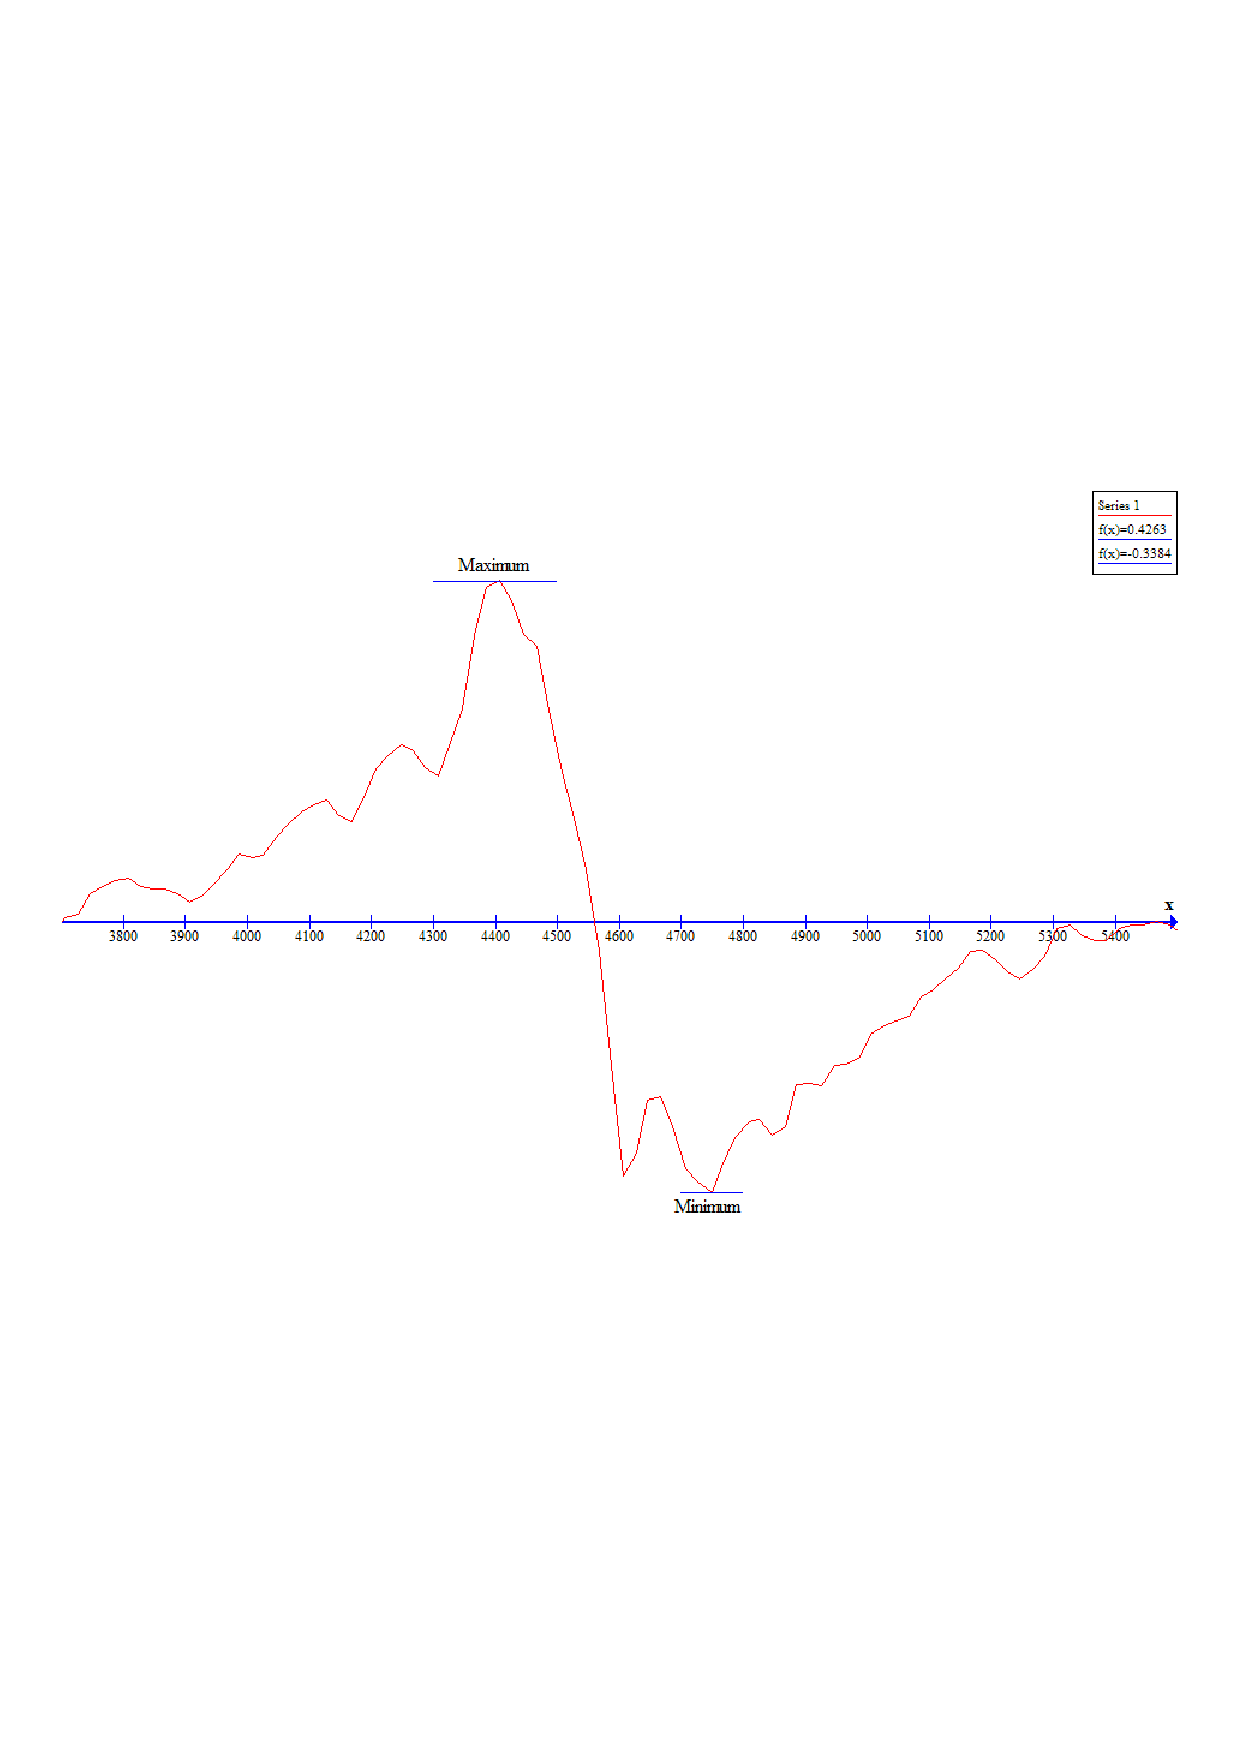
\includegraphics[trim=0 8cm 0cm 8cm, clip,scale=0.5]{media/peak-detection}
\caption{Peak detection finding one step.}
\label{figure:peak-detection}
\end{figure}

\begin{figure}[H]
\centering
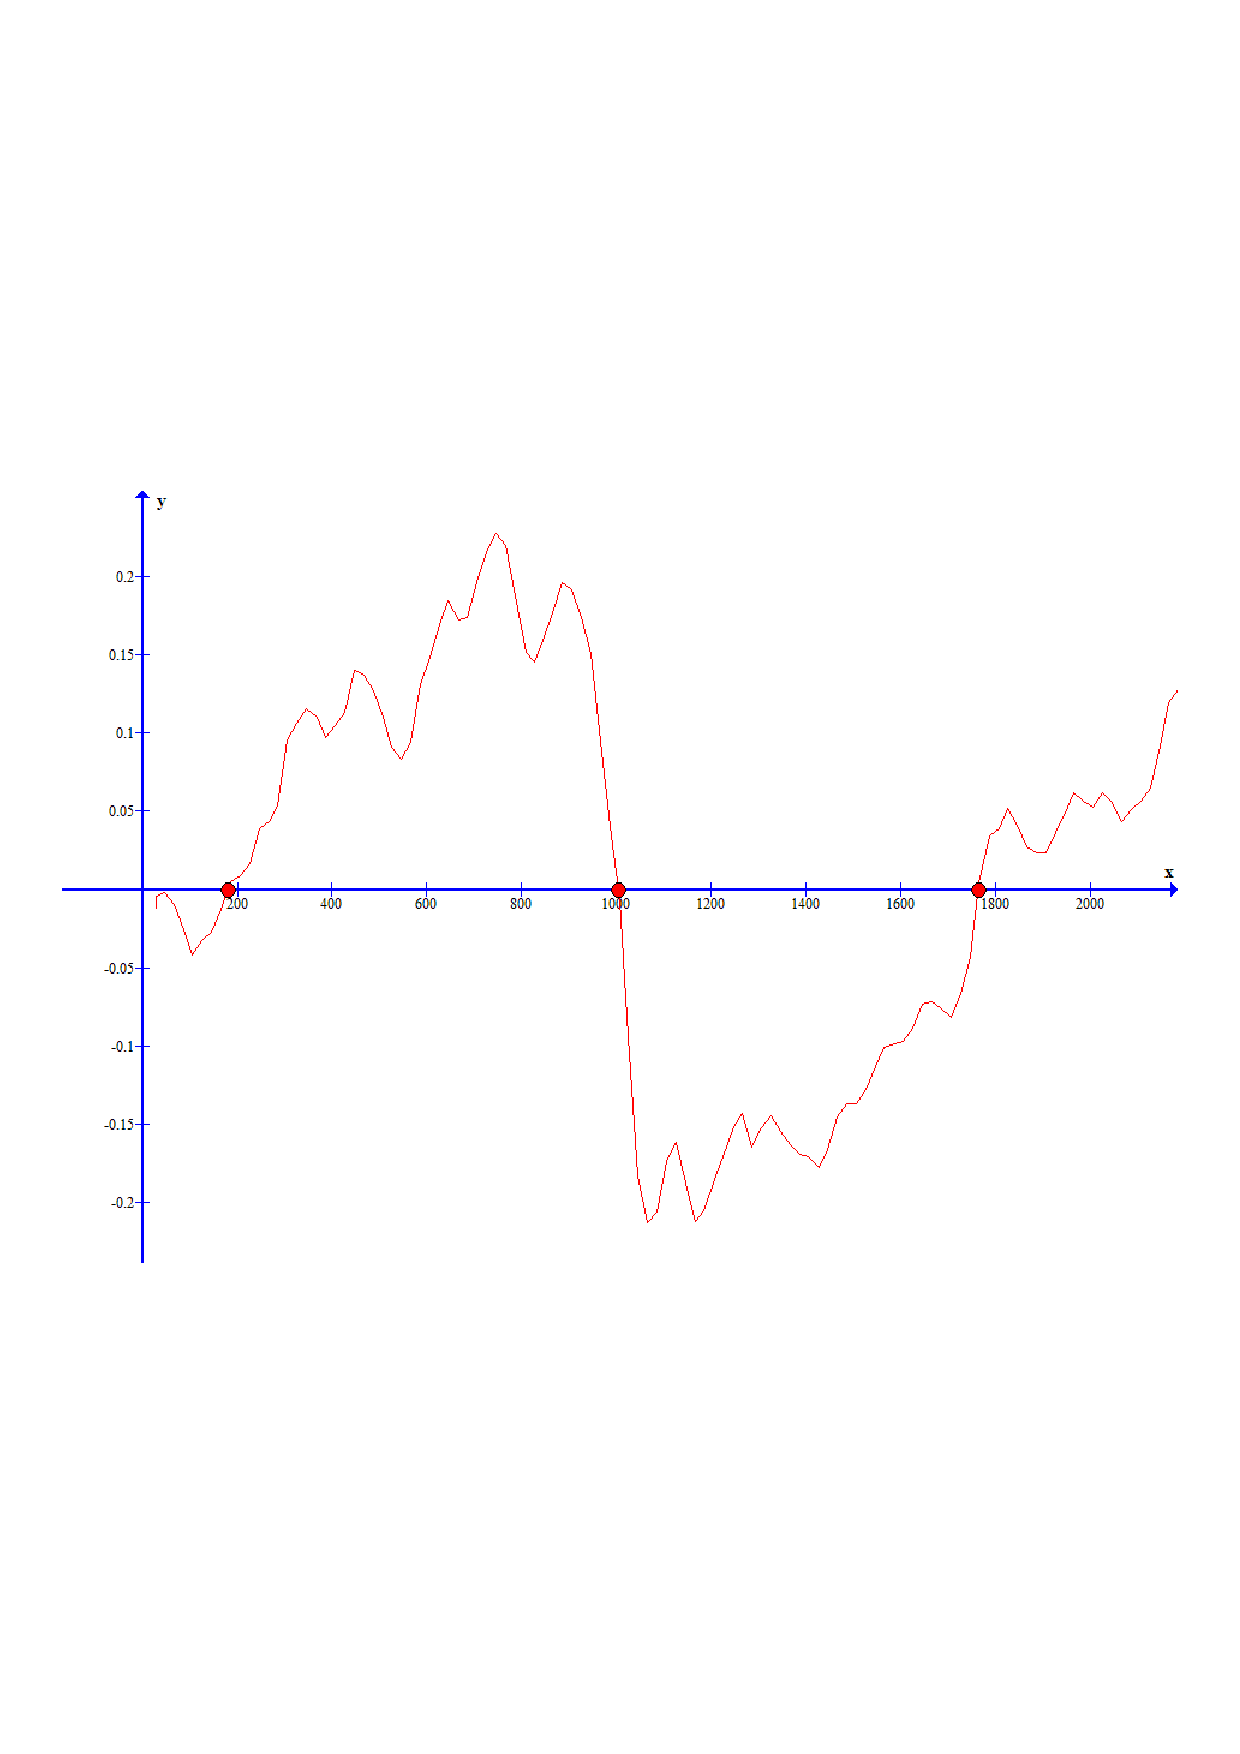
\includegraphics[trim=0 8cm 0cm 8cm, clip,scale=0.5]{media/zero-crossing}
\caption{Zero crossing determining a step.}
\label{figure:zero-crossing}
\end{figure}

After finding the step, the step length can be determined by a linear combination of walking velocity and variance of the accelerometer, \eqref{eq:steplength}. \fxnote{er usikre på denne formel, vi mener v er noise fra accelerometer men er ikke sikker}
The walking distance, \eqref{eq:walkingdistance}, is the accumulated value of all the steps, which were found using the previously described algorithms and the step length equation.
\begin{equation}\label{eq:steplength}
	Step length = \alpha * f + \beta * v + \gamma \\
\end{equation}
\begin{equation}\label{eq:walkingdistance}
	Walking distance = \sum\limits_{i=1}^{n} (\alpha * f_i + \beta * v_i + \gamma)
\end{equation}
where,
\begin{itemize}
	\item[$\alpha , \beta$] is weights of walking parameters.
	\item[$\gamma$] is a constant.
	\item[$f_i$] is the walking velocity of the i-th step.
	\item[$v_i$] is the acceleration variance of the i-th step.
\end{itemize}

These formulas can be erroneous as the location of the phone can change which creates bad inputs in the calculation of the walking distance.
Determining the location of the phone is therefore important in pedestrian dead reckoning i.e if it is in the pocket, bag, or hand. But as this project is constraint to having the phone in a fixed position, phone location awareness as it is not necessary.